\section{Turmeric}
\label{sec:turmeric}

\begin{spice}\label{spice:turmeric}
\textsc{Turmeric} \hfill \href{https://powo.science.kew.org/taxon/796451-1}{POWO} \\
\textbf{English:} \textit{turmeric}. 
\textbf{Arabic:} {\arabicfont{كركم}} \textit{kurkum}. 
\textbf{Chinese:} {\tradchinesefont{薑黃}} \textit{jiānghuáng} [ginger-yellow]; 黃薑 \textit{huángjiāng} [yellow-ginger]. 
\textbf{Hungarian:} \textit{kurkuma}.  \\
\noindent{\color{black}\rule[0.5ex]{\linewidth}{.5pt}}
\begin{tabular}{@{}p{0.25\linewidth}@{}p{0.75\linewidth}@{}}
Plant species: & \taxonn{Curcuma longa}{L.} (syn. \taxonn{Curcuma domestica}{Valeton}) \\
Family: & \textit{Zingiberaceae} \\
part used: & rhizome \\
Region of origin: & India \\
Cultivated in: & China; Honduras; India; Indonesia; Jamaica \\
Color: & orange-yellow \\
\end{tabular}
\end{spice}

\begin{figure}[!ht]
	\vspace{-4ex}
	\centering
	\subfloat{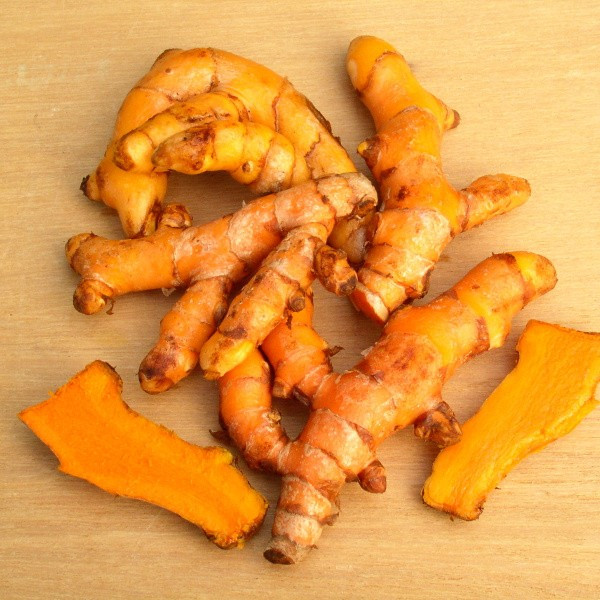
\includegraphics[width=0.3\linewidth]{imgs/spices/turmeric-4.jpg}}
	\hfill
	\subfloat{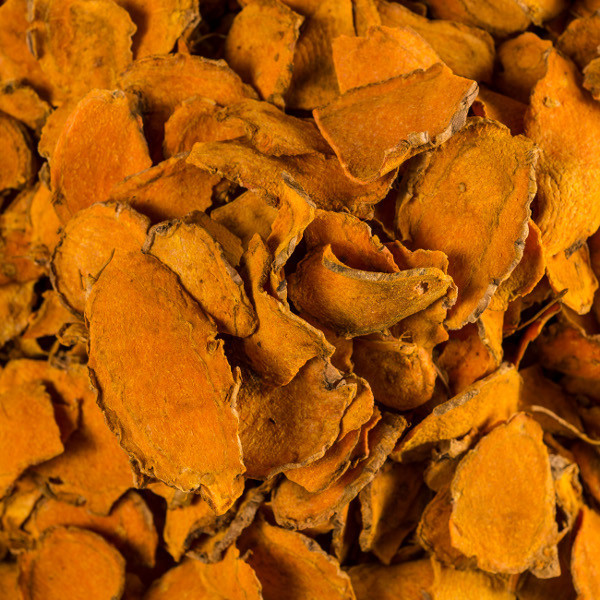
\includegraphics[width=0.3\linewidth]{imgs/spices/turmeric-1.jpg}}
	\hfill
	\subfloat{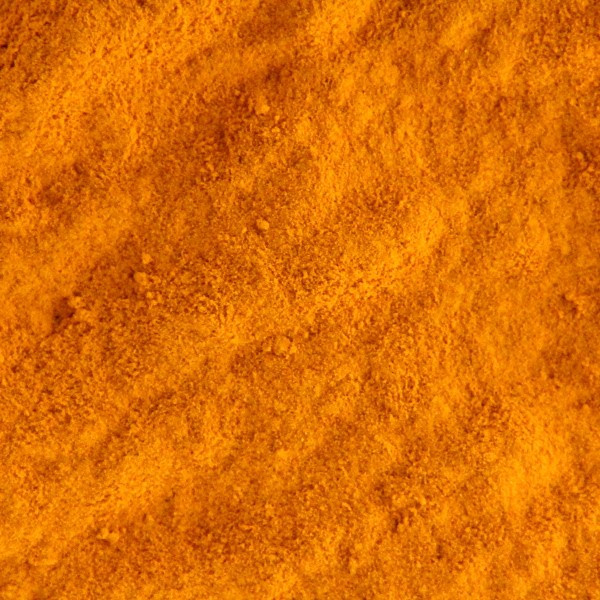
\includegraphics[width=0.3\linewidth]{imgs/spices/turmeric-3.jpg}}
	\caption{ \taxon{Curcuma longa}. Credits: Aromatiques.}
	\label{fig:turmeric_imgs}
\end{figure}

Turmeric is a spice obtained from the dried rhizomes of \taxon{Curcuma longa}, an aromatic plant closely related, and very similar to ginger (\cref{sec:ginger}). Commercial turmeric can be found in the shape of finger-like knobs, slices, and most commonly, powder, as it can be seen on \cref{fig:turmeric_imgs}. Turmeric is an important ancient spice, medicine, dye, and ritual substance, and it turns everything it touches yellow.

\subsection{The Botany, Origins, and Cultivation of Turmeric}


% Description The rhizomes are finger-like and bright orange inside when freshly cut but bright yellow when dried and orange-yellow when powdered. They are easily confused with the bright orange but more conical Indonesian mango ginger (C. mangga) or the similarly shaped but pale yellow mango ginger (C. amada).1 Wild turmeric (C. aromatica) is also used as a source of dye.2 The stoloniferous zedoary or e-zhu (C. zedoaria) is an alternative source of turmeric in China. the plant A leafy, stemless, ginger-like plant with large, oblong leaves and attractive yellow and white flowers borne in oblong clusters. origin Turmeric is an ancient cultigen not found in the wild but is believed to be indigenous to southern Asia (possibly India). It has been used as a spice and dye since ancient times and is also important in religious rites and traditional customs. From India the plant is believed to have spread to Southeast Asia, the Far East and Polynesia (as far as Fiji) and much later to tropical America.1 cultivation Turmeric is a sterile triploid and is propagated vegetatively by division of the branched rhizomes. It requires a tropical climate and high rainfall. harvesting The rhizomes are dug up when mature, after which they may be boiled, dried and powdered to produce turmeric powder. India is the most important producer, with nearly 350 000 tons per year but smaller amounts are also produced in Bangladesh, Pakistan and various South and Southeast Asian countries.1 culinary uses Turmeric is best known as the spice that gives curry powder and mustard

% powder their bright orange or yellow colour. The fresh rhizomes, powdered rhizomes or extracts are important ingredients of Indian and Asian cooking. They are added to a wide range of dishes, not only for colour but also for flavour, including meat, fish, vegetables and rice dishes. A wellknown example is Malaysian yellow rice (nasi kunyit), eaten on ceremonial or festive occasions and the origin of the geelrys (“yellow rice”) of Cape cookery. Turmeric is used as a natural food dye in many food products, including mustard sauces, Worcestershire sauce, sandwich spread, butter, cheese, beverages, dairy products, drinks, confectionery, pickles and soup powders. Mango ginger has the flavour and aroma of raw mango and is used in curries and pickles.1 Indonesian mango ginger is similar to mango ginger in flavour and uses. Flavour compounDs The bright yellow colour is due to pigments (curcuminoids) of which curcumin is the main compound.3 The essential oil has a warm, spicy, earthy and slightly bitter flavour and contains mainly sesquiterpenes, of which ar-turmerone and turmerone are the major compounds.4 notes Curcumin has a wide range of medicinal properties.3

% 1. Nayar, N.M., Ravindran, P.N. 1995. Herb spices. In: Smartt, J., Simmonds, N.W. (Eds), Evolution of crop plants (2nd ed.), pp. 491–494. Longman, London. 2. Mabberley, D.J. 2008. Mabberley’s plant-book (3rd ed.). Cambridge University Press, Cambridge. 3. Esatbeyoglu, T., Huebbe, P., Ernst, I.M.A., Chin, D., Wagner, A.E., Rimbach, G. 2012. Curcumin—from molecule to biological function. Angewandte Chemie, International Edition, 51: 5308–5332. 4. Gopalan, B., Goto, M., Kodama, A., Hirose, T. 2000. Supercritical carbon dioxide extraction of turmeric (Curcuma longa). Journal of Agricultural and Food Chemistry 48: 2189.

\subsection{The History of Turmeric}

\subsection{The Names of Turmeric}
\label{sec:names_of_turmeric}

\subsubsection{English}

\begin{table}[!ht]
\centering
\begin{tabularx}{\textwidth}{@{}l>{\itshape \small}lL>{\small}l@{}}
\toprule
\textbf{\#} & \multicolumn{1}{l}{\textbf{Species}} & \multicolumn{1}{l}{\textbf{Name}} & \multicolumn{1}{l}{\textbf{Source}} \\
\midrule
1	& Curcuma longa	& curcuma	& \textcite{oed} \\
2	& Curcuma longa	& Indian saffron	& \textcite{oed} \\
\textbf{3}	& \textbf{Curcuma longa}	& \textbf{turmeric}	& \textbf{\textcite{van_wyk_culinary_2014}} \\
\bottomrule
\end{tabularx}
\caption{Various names for turmeric in English.}
\label{table:names_turmeric_en}
\end{table}



\begin{etymology}\label{ety:turmeric}
English \textit{turmeric} `turmeric'
< French \textit{terre mérite} `turmeric'
< Medieval Latin \textit{terra merita} `turmeric'\footnote{}
\end{etymology}

\subsubsection{Arabic}

\begin{table}[!ht]
\centering
\begin{tabularx}{\textwidth}{@{}l>{\itshape \small}lr>{\itshape}lL>{\small}l@{}}
\toprule
\textbf{\#} & \multicolumn{1}{l}{\textbf{Species}} & \multicolumn{1}{l}{\textbf{Name}} & \multicolumn{1}{l}{\textbf{Tr.}} & \multicolumn{1}{l}{\textbf{Gloss}} & \multicolumn{1}{l}{\textbf{Source}} \\
\midrule
1	& Curcuma longa	& أصابع صفر	& aṣābiʿ ṣufr	& yellow fingers	& \textcite{wikipedia} \\
2	& Curcuma longa	& هرد	& hurd	& 	& \textcite{amar_arabian_2017} \\
\textbf{3}	& \textbf{Curcuma longa}	& \textbf{كركم}	& \textbf{kurkum}	& \textbf{phonetic}	& \textbf{\textcite{amar_arabian_2017}} \\
4	& Curcuma longa	& شجرة الخطاطيف	& shajarat al-khaṭāṭīf	& 	& \textcite{amar_arabian_2017} \\
5	& Curcuma longa	& زعفران هندي	& zaʿfarān hindī	& Indian saffron	& \textcite{amar_arabian_2017} \\
6	& Curcuma longa	& عقدة صفراء	& ʿuqda ṣafrā'	& yellow knob	& \textcite{baalbaki_-mawrid_1995} \\
7	& Curcuma longa	& عروق صفر	& ʿurūq ṣufr	& 	& \textcite{amar_arabian_2017} \\
\bottomrule
\end{tabularx}
\caption{Various names for turmeric in Arabic.}
\label{table:names_turmeric_ar}
\end{table}



\begin{etymology}\label{ety:kurkum}
\textbf{Arabic} {كركم} \textit{kurkum} `turmeric; saffron'; cf. cognates Hebrew \he{כַּרְכֹּום} \textit{karkom}; Aramaic \he{כּוּרְכְּמָא}/\sy{ܟܽܘܪܟܡܳܐ} \textit{kurkmā}; Akkadian \cu{𒌑𒆪𒄀𒆸𒈾} \textit{kurkanū}
<\textss{?} \textbf{Sanskrit} {कुङ्कुम } \textit{kuṅkuma} `saffron'\footnote{\textcite[s.v. kwrkm]{cal}; \textcite{guthrie_trade-language_2009}}
\end{etymology}

\subsubsection{Chinese}

\begin{table}[!ht]
\centering
\begin{tabularx}{\textwidth}{@{}l>{\itshape \small}ll>{\itshape}lL>{\small}l@{}}
\toprule
\textbf{\#} & \multicolumn{1}{l}{\textbf{Species}} & \multicolumn{1}{l}{\textbf{Name}} & \multicolumn{1}{l}{\textbf{Tr.}} & \multicolumn{1}{l}{\textbf{Gloss}} & \multicolumn{1}{l}{\textbf{Source}} \\
\midrule
1	& Curcuma longa	& \tradchinesefont{寶鼎香}	& bǎodǐngxiāng	& treasure-cauldron-spice?	&  \\
2	& Curcuma longa	& \tradchinesefont{黃薑}	& huángjiāng	& yellow-ginger	& \textcite{defrancis_abc_2003} \\
\textbf{3}	& \textbf{Curcuma longa}	& \textbf{\tradchinesefont{薑黃}}	& \textbf{jiānghuáng}	& \textbf{ginger-yellow}	& \textbf{\textcite{kleeman_oxford_2010}} \\
\bottomrule
\end{tabularx}
\caption{Various names for turmeric in Chinese.}
\label{table:names_turmeric_zh}
\end{table}



\begin{etymology}\label{ety:jianghuang}
\textbf{Mandarin Chinese} \traditionalchinesefont{薑黃} \textit{jiānghuáng} `turmeric', \textit{jiang} `ginger' + \textit{huang} `yellow'\footnote{\textcite[856]{kleeman_oxford_2010}}
\end{etymology}

\subsubsection{Summary}

\begin{table}[!ht]
\centering
\begin{tabularx}{\textwidth}{@{}ll>{\itshape}lLl>{\small}l@{}}
\toprule
\textbf{\#} & \textbf{Language} & \multicolumn{1}{l}{\textbf{Term}} & \textbf{Gloss} & \textbf{Loan} & \multicolumn{1}{l}{\textbf{Source}} \\
\midrule
1	& English	& curcuma	& 	& yes	& \textcite{oed} \\
2	& English	& Indian saffron	& 	& no	& \textcite{oed} \\
3	& English	& turmeric	& 	& yes	& \textcite{oed} \\
\midrule
1	& Arabic	& hurd	& 	& yes	& \textcite{lane_arabic-english_1863} \\
2	& Arabic	& kurkum	& phonetic	& yes	& \textcite{wehr_dictionary_1976} \\
3	& Arabic	& ʿuqda ṣafrā'	& yellow knob	& no	& \textcite{baalbaki_-mawrid_1995} \\
\midrule
1	& Chinese	& huángjiāng	& yellow-ginger	& no	& \textcite{defrancis_abc_2003} \\
2	& Chinese	& jiānghuáng	& ginger-yellow	& no	& \textcite{kleeman_oxford_2010} \\
\bottomrule
\end{tabularx}
\caption{Conventionalized names for turmeric in English, Arabic, and Chinese, found in dictionaries.}
\label{table:names_turmeric}
\end{table}

















% Cantonese: 黃薑 (wong4 goeng1)

% EE:
% (powder made from) the root-stock of the East Indian plant, used in curry powder, etc. XVI. Early forms also tarmaret, tormarith, which appear to be — F. terre mérite, modL. terra merita, of unkn. orig.; the ending shows assim. to -IC.

% OE:
% pungent powder made from the root of an East Indian plant, 1530s, altered from Middle English turmeryte (early 15c.), which is of uncertain origin. "Middle English Compendium" compares Medieval Latin terra merita (16c.), French terre mérite (17c.), literally "worthy earth," though the reason why it would be called this is obscure. Klein suggests it might be a folk-etymology corruption of Arabic kurkum "curcuma, saffron."

% MW:
% modification of Middle French terre merite saffron, from Medieval Latin terra merita, literally, deserving or deserved earth
% First Known Use: 15th century (sense 1a(1))

% AH:
% [Alteration of Middle English termeryte; akin to French terre mérite and New Latin terra merita, turmeric (New Latin, from Latin terra, earth; see ters- in the Appendix of Indo-European roots + merita, feminine past participle of merēre, to deserve; see (s)mer-2 in the Appendix of Indo-European roots).]

% WK:
% From Middle English turmeryte, tarmaret, of uncertain origin. Possibly from Old French terre mérite (“deserving earth”). According to Klein, possibly corrupted from Arabic كُرْكُم (kurkum, “Curcuma”). 